\chapter{Matrices as Transformations}
Recall that a \emph{function}, informally, is a rule that takes an input and produces an output. 

For example, we know the common function $f(x) = x^3$ takes the input and cubes it, such that the result is $x \times x \times x$. Inputting $x=3$ outputs $f(3) = 27$. 

In Linear Algebra, we can think of matrices as a type of function. Recall our systems of matrices equation,
$$A\vec{x}=\vec{b}$$
We can rearrange this to look closer to function notation:
$$\vec{b}=A\vec{x}$$
We can change our input vector $\vec{x}$, which directly affects the output variable $\vec{b}$. 

Recall our subspace diagram; the matrix $A$, which is size $m\times n$, takes the input vectors $\vec{x} \in \mathbb R^n$, and transforms them to the output $\vec{b} \in \mathbb R^m$.


The transformation $T$ is said to map from the reals of $n$ to the reals of $m$, such that: $T: \mathbb R^{n}\to \mathbb R^m$
\begin{itemize}
    \item $\mathbb R^n$ is called the \textbf{domain}
    \item $\mathbb R^m$ is called the \textbf{codomain}
\end{itemize}

\begin{figure}[H]
    \centering
    %drawing made in mathcha 
    \tikzset{every picture/.style={line width=0.75pt}} %set default line width to 0.75pt        

    \begin{tikzpicture}[x=0.75pt,y=0.75pt,yscale=-1,xscale=1]
    %uncomment if require: \path (0,300); %set diagram left start at 0, and has height of 300

    %Curve Lines [id:da9612466263999061] 
    \draw    (106,59) .. controls (145.6,29.3) and (213.62,28.02) .. (252.82,58.08) ;
    \draw [shift={(254,59)}, rotate = 218.48] [color={rgb, 255:red, 0; green, 0; blue, 0 }  ][line width=0.75]    (10.93,-3.29) .. controls (6.95,-1.4) and (3.31,-0.3) .. (0,0) .. controls (3.31,0.3) and (6.95,1.4) .. (10.93,3.29)   ;
    %Curve Lines [id:da47200980654646296] 
    \draw    (106.47,82.73) .. controls (139.39,120.02) and (217.54,120.4) .. (253,81) ;
    \draw [shift={(105,81)}, rotate = 50.63] [color={rgb, 255:red, 0; green, 0; blue, 0 }  ][line width=0.75]    (10.93,-3.29) .. controls (6.95,-1.4) and (3.31,-0.3) .. (0,0) .. controls (3.31,0.3) and (6.95,1.4) .. (10.93,3.29)   ;


    % Text Node
    \draw (108.96,68) node  [xscale=0.8,yscale=0.8]  {$\mathbb{R}^{n}$};
    % Text Node
    \draw (255.96,68) node  [xscale=0.8,yscale=0.8]  {$\mathbb{R}^{m}$};
    % Text Node
    \draw (94,59) node [anchor=east] [inner sep=0.75pt]  [xscale=0.8,yscale=0.8]  {$N( A)$};
    % Text Node
    \draw (94,79) node [anchor=east] [inner sep=0.75pt]  [xscale=0.8,yscale=0.8]  {$R( A)$};
    % Text Node
    \draw (271.87,59) node [anchor=west] [inner sep=0.75pt]  [xscale=0.8,yscale=0.8]  {$N\left( A^{\top }\right)$};
    % Text Node
    \draw (272.81,79) node [anchor=west] [inner sep=0.75pt]  [xscale=0.8,yscale=0.8]  {$C( A)$};
    % Text Node
    \draw (178.9,19.84) node  [xscale=0.8,yscale=0.8]  {$\underset{m\times n}{A}$};
    % Text Node
    \draw (176.9,127.84) node  [xscale=0.8,yscale=0.8]  {$\underset{n\times m}{A^{\top }}$};
    % Text Node
    \draw (139,119) node [anchor=east] [inner sep=0.75pt]  [xscale=0.8,yscale=0.8]  {$ \begin{array}{l}
    N( A) \ \perp \ R( A)\\
    N( A) \ \cdot \ R( A) \ =\ 0
    \end{array}$};
    % Text Node
    \draw (371,122) node [anchor=east] [inner sep=0.75pt]  [xscale=0.8,yscale=0.8]  {$ \begin{array}{l}
    N\left( A^{\top }\right) \ \perp \ C( A)\\
    N\left( A^{\top }\right) \ \cdot \ C( A) \ =\ 0
    \end{array}$};


    \end{tikzpicture}
    \label{fig:transformationDiagram}
\end{figure}

Let's call the transformation $T$, such that 
$$T : \mathbb R^n \to \mathbb R^m$$

We can rewrite our transformation with matrix $A$ 
$$T(\vec x) = A\vec x$$

A matrix transformation is completely determined by where it sends the \emph{standard basis vectors}. Each column of $A$ is the image of a basis vector under the transformation, and every output vector is a linear combination of these columns.

Consequently, the column space of $A$ represents the full set of possible outputs of the transformation.
\subsection{The Identity Transformation}
For this chapter, we will restrict our transformations to $\mathbb R^2 \rightarrow \mathbb R^2$, such that our matrix is $2 \times 2$. This will help calculations be simpler and also will allow us to make easy to follow transformation diagrams. 

Let's take the simplest transformation; the \emph{identity transformation}\index{identity transformation}. Take the matrix:
$$I = \begin{bmatrix}1 & 0 \\ 0 & 1\end{bmatrix}$$

Every vector in the subspace of $\mathbb R^n$ \textbf{stays where it is}.
\begin{itemize}
    \item $e_1$ stays $e_1$
    \item $e_2$ stays $e_2$
\end{itemize}

\textit{Every vector stays where it originally started in this transformation.} In a way, no transformation is truly applied. 

Under the identity transformation, nothing moves. We still get something very important out of this: the vector $\vecb{1 \\ 1}$ can be written as a combination of the basis vectors:
$$\vecb{1 \\ 1} = 1\vec e_1 + 1\vec e_2$$
When a linear transformation is applied, the way a vector is built from the basis vectors does not change, but \emph{rather the direction of the basis vectors}.
\begin{figure}[H]
    \centering
    \begin{subfigure}[b]{0.45\textwidth}
        \centering
        \includegraphics[width=\textwidth]{identity_transform_basis.png}
        \caption{Identity vectors before transformation}
        \label{fig:identity_transform_a}
    \end{subfigure}
    \hfill
    \begin{subfigure}[b]{0.45\textwidth}
        \centering
        \includegraphics[width=\textwidth]{identity_transform.png}
        \caption{Identity vectors after transformation (no change)}
        \label{fig:identity_transform_b}
    \end{subfigure}
    \caption{An identity transformation acting on basis vectors.}
    \label{fig:identity_transform}
\end{figure}


A linear transformation acts on $\vec{x}$ by acting on each basis vector individually:
$$A\vec x = x_1A\vec e_1 + x_2A\vec e_2$$

such that any coefficient $x_1$ and $x_2$ are unchanged, while $e_1$ and $e_2$ are transformed. 

Our chapter will also take a look at transforming a simple house. Here is the house before any transformations (or, with the identity transformation applied):
\begin{figure}[H]
    \centering
    \includegraphics[width=0.8\textwidth]{house_identity.png}
    \caption{A simple house before any transformations.}
    \label{fig:house_identity}
\end{figure}
Linear transformations preserve linear combinations while \emph{altering the directions that define the coordinate system}.

In the next example, we will apply a non-identity matrix and observe how transforming the basis vectors reshapes the entire space. Each figure will show a grid of points in $\mathbb R^2$ alongside the resulting transformed points after applying the matrix transformation. We encourage you to play with the python script \texttt{transforms.py} to see how different matrices affect the transformation. Also, we will limit our view to a square region from $(-2, -2)$ to $(2, 2)$ and only use $2 \times 2$ matrices for simplicity.

\subsection{Scaling and Shearing}
\index{scaling}
\section{Scaling}
Now, let's try scaling up and down the basis vectors. Consider the matrix:
\[A = \begin{bmatrix} 2 & 0 \\ 0 & 2 \end{bmatrix}\]
This matrix will scale both the $e_1$ and $e_2$ vectors by a factor of 2, effectively doubling their lengths.

\begin{figure}[H]
    \centering
    \includegraphics[width=0.8\textwidth]{grid_scaling_2x.png}
    \caption{The effect of the scaling transformation $A = \begin{bmatrix} 2 & 0 \\ 0 & 2 \end{bmatrix}$ on a grid of points.}
    \label{fig:grid_scaling_2x}
\end{figure}

What happens to our house? Well, each part of the house is transformed linearly by 2, a linear \emph{scaling}.
\begin{figure}[H]
    \centering
    \includegraphics[width=0.8\textwidth]{house_scaling_2x.png}
    \caption{The effect of the scaling transformation $A = \begin{bmatrix} 2 & 0 \\ 0 & 2 \end{bmatrix}$ on a simple house.}
    \label{fig:house_scaling_2x}
\end{figure}

This tells us that the transformation $A$ is a scaling transformation, which stretches the space by a factor of 2 in both directions. What do you think happens if we scale by a factor of $\frac{1}{2}$ instead? Try it out!
\begin{figure}[H]
    \centering
    \includegraphics[width=0.8\textwidth]{house_scaling_0.5x.png}
    \caption{The effect of the scaling transformation $A = \begin{bmatrix} 0.5 & 0 \\ 0 & 0.5 \end{bmatrix}$ on a simple house.}
    \label{fig:house_scaling_0.5x}
\end{figure}
This, as expected, shrinks the house by a factor of $\frac{1}{2}$ in both directions.


Now, let's try scaling up \emph{only one} of the basis vectors. Consider the matrix:
\[A_{\textrm{rightward shear}} = \begin{bmatrix} 1 & 0 \\ 0 & 2 \end{bmatrix}\]

This matrix will scale the $e_1$ vector by a factor of 1 (no change) and the $e_2$ vector by a factor of 2 (doubling its length).

Applying this transformation to the basis vectors produces this result:
\begin{figure}[H]
    \centering
    \includegraphics[width=0.8\textwidth]{e2scaled.png}
    \caption{The effect of the scaling transformation $A = \begin{bmatrix} 1 & 0 \\ 0 & 2 \end{bmatrix}$ on the standard basis vectors.}
    \label{fig:e2scaled}
\end{figure}

Applying this transformation to our house:
\begin{figure}[H]
    \centering
    \includegraphics[width=0.8\textwidth]{house_shear_k2.0.png}
    \caption{The effect of the shearing transformation $A = \begin{bmatrix} 1 & 2 \\ 0 & 1 \end{bmatrix}$ on a simple house.}
    \label{fig:house_shear_k2.0}
\end{figure}
\section{Reflections} 
\index{reflections}
How would we do reflections across a given axis? Let's think about what happens to each point. Reflecting individual points is the same as reflecting the basis vectors, since every point is a linear combination of the basis vectors.

\subsection{Reflection across the x-axis}
For a reflection across the x-axis, the y-values of each point change sign, while the x-values stay the same. $$(x, y) \mapsto (x, -y)$$ 

This means that $e_1$ stays $e_1$, while $e_2$ becomes $-e_2$. This allows us to rewrite a $2 \times 2$ matrix for this transformation:

\[A_{x-axis} = \begin{bmatrix} 1 & 0 \\ 0 & -1 \end{bmatrix}\]

Below is a pink test vector $\vecb{1 \\ 1}$ and its transformation in purple, which is $\vecb{1 \\ -1}$.
\begin{figure}[H]
    \centering
    \includegraphics[width=\textwidth]{refl_x_axis.png}
    \caption{The effect of reflecting across the x-axis. Added is the vector $\vecb{1 \\ 1}$ and its transformation in purple.}
    \label{fig:refl_x_axis}
\end{figure}

Also, we can reflect our house across the x-axis. We will see a difference in where the chimney, roof, and door are located. 
\begin{figure}[H]
    \centering
    \includegraphics[width=0.8\textwidth]{house_reflection_x_axis.png}
    \caption{The effect of reflecting a house across the x-axis. Red house is the transformed house, while the black house is the original.}
    \label{fig:house_reflection_x_axis}
\end{figure}

\subsection{Reflection across the y-axis}
What if we want to reflect across the y-axis instead? In this case, the x-values of each point change sign, while the y-values stay the same. As a function of points, this is
$$(x, y) \mapsto (-x, y)$$

Our basis vector $e_1$ becomes $-e_1$, while $e_2$ stays $e_2$. This allows us to rewrite a matrix for this transformation:
\[A_{y-axis} = \begin{bmatrix} -1 & 0 \\ 0 & 1 \end{bmatrix}\]
\begin{figure}[H]
    \centering
    \includegraphics[width=\textwidth]{refl_y_axis.png}
    \caption{The effect of reflecting across the y-axis. Added is the vector $\vecb{1 \\ 1}$ and its transformation in purple.}
    \label{fig:refl_y_axis}
\end{figure}

Notice that it is simlar to the effect of a selfie, where the left and right sides are flipped. This may be more noticable in the house transformation, where the door and chimney are on the opposite sides of the house.
\begin{figure}[H]
    \centering
    \includegraphics[width=0.8\textwidth]{house_reflection_y_axis.png}
    \caption{The effect of reflecting a house across the y-axis.}
    \label{fig:house_reflection_y_axis}
\end{figure}

Note that the red house is still upright, but the left and right sides are flipped. This makes sense, since the y-values of the points are unchanged, while the x-values flip signs.

\subsection{Reflection across the lines $y=x$ and $y=-x$}
As we have seen, there are two standard lines important for inverse functions: $y=x$ and $y=-x$. We can also reflect across these lines.

The line $y=x$ is the line where the x and y values are equal. When we reflect across this line, the x and y values swap places. As a function of points, this is
$$(x, y) \;\mapsto\; (y, x)$$
Since each point swaps places, the basis vectors also swap places. $e_1$ becomes $e_2$, while $e_2$ becomes $e_1$. This allows us to rewrite a matrix for this transformation:
\[A_{y=x} = \begin{bmatrix} 0 & 1 \\ 1 & 0 \end{bmatrix}\]

Let's look at our house picture, reflected across the line $y=x$. Notice that the house is flipped across the line, such that the roof is now on the bottom and the door is on top.

\begin{figure}[H]
    \centering
    \includegraphics[width=0.8\textwidth]{house_reflection_y_equals_x_axis.png}
    \caption{The effect of reflecting a house across the line $y=x$.}
    \label{fig:house_reflection_y_equals_x_axis}
\end{figure}

The line $y=-x$ is the line where the x and y values are equal but with opposite signs. When we reflect across this line, the x and y values swap places and flip signs. As a function of points, this is
$$(x, y) \;\mapsto\; (-y, -x)$$
Not only do the x and y values swap places, but they also flip signs. This means that $e_1$ becomes $-e_2$, while $e_2$ becomes $-e_1$. This allows us to rewrite a matrix for this transformation, where
\[A_{y=-x} = \begin{bmatrix} 0 & -1 \\ -1 & 0 \end{bmatrix}\]
\begin{figure}[H]
    \centering
    \includegraphics[width=0.8\textwidth]{house_reflection_y_equals_neg_x_axis.png}
    \caption{The effect of reflecting a house across the line $y=-x$.}
    \label{fig:house_reflection_y_equals_neg_x_axis}
\end{figure}


% Note for future writers: I am not doing y=mx reflections as they are more complex and I am already hitting a complexity limit for linear alg.
\section{Rotations}
%FIXME content not written just graphs
% FIXME derived rotation matrices from trig functions but bring back y=x y=-x
Those past four transformations (\ref{fig:house_reflection_x_axis}, \ref{fig:house_reflection_y_axis}, \ref{fig:house_reflection_y_equals_x_axis}, \ref{fig:house_reflection_y_equals_neg_x_axis}) all had something similar %fixme

What if we want to rotate our house? We can also do this with a matrix transformation. It may look similar to the reflections, but it is not the same. Let's track our basis vectors to see where they end up:
$$\vecb{1\\0}\mapsto\vecb{0\\1}, \qquad \vecb{0\\1}\mapsto\vecb{-1\\0}$$

From this, we can write the matrix for a $90^\circ$ rotation clockwise:
\[A_{90^\circ}^{\textrm{cw}} = \begin{bmatrix} 0 & 1 \\ -1 & 0 \end{bmatrix}\]

What about a $90^\circ$ rotation counterclockwise? We can track our basis vectors again:
$$\vecb{1\\0}\mapsto\vecb{0\\-1}, \qquad \vecb{0\\1}\mapsto\vecb{1\\0}$$

And so the matrix for a $90^\circ$ rotation counterclockwise is:
\[A_{90^\circ}^{\textrm{ccw}} = \begin{bmatrix} 0 & -1 \\ 1 & 0 \end{bmatrix}\]

However, we have learned trigonometric functions that result in these values. We know that at $90^\circ$, $\cos(90^\circ) = 0$ and $\sin(90^\circ) = 1$. So we could say:
\[A_{90^\circ}^{\textrm{cw}} = \begin{bmatrix} \cos(90^\circ) & \sin(90^\circ) \\ -\sin(90^\circ) & \cos(90^\circ) \end{bmatrix}\]
Note that this aligns with our \emph{polar} coordinate system where cosine is the x-value and sine is the y-value. 

For a counterclockwise rotation of $90^\circ$, we have:
\[A_{90^\circ}^{\textrm{ccw}} = \begin{bmatrix} \cos(90^\circ) & -\sin(90^\circ) \\ \sin(90^\circ) & \cos(90^\circ) \end{bmatrix}\]

But, we can generalize this to any angle $\theta$ instead of just $90^\circ$. For a clockwise rotation by $\theta$, we have:
\[A_{\theta}^{\textrm{cw}} = \begin{bmatrix} \cos(\theta) & \sin(\theta) \\ -\sin(\theta) & \       cos(\theta) \end{bmatrix}\]
And for a counterclockwise rotation by $\theta$, we have:
\[A_{\theta}^{\textrm{ccw}} = \begin{bmatrix} \cos(\theta) & -\sin(\theta) \\ \sin(\theta) & \cos(\theta) \end{bmatrix}\]

Note how similar they are! The only difference is the sign of the sine values. Sine is an odd function, which means that $\sin(-\theta) = -\sin(\theta)$, so the sign of the sine values determines the direction of rotation.

Let's see what happens when we apply a $30^\circ$ clockwise and counterclockwise rotation to our house. We can calculate the matrix for this transformation using the cosine and sine values for $30^\circ$:
\begin{figure}[H]
    \centering
    \begin{subfigure}[b]{\textwidth}
        \centering
        \includegraphics[width=\textwidth]{house_rotation_cw_30deg.png}
        \caption{30 degree clockwise rotation}
        \label{fig:30degcw}
    \end{subfigure}
    \hfill
    \begin{subfigure}[b]{\textwidth}
        \centering
        \includegraphics[width=\textwidth]{house_rotation_ccw_30deg.png}
        \caption{30 degree counterclockwise rotation}
        \label{fig:30degccw}
    \end{subfigure}
    \caption{The effect of 30 degree rotations on our house.}
    \label{fig:30deg_rotations}
\end{figure}

% Writers note: Not talked about is applying multiple transformations in sequence, which would be a good follow up topic. I feel like it is not necessary for our linear algebra foundation, but could be a good extension. Again, this is a high school level text. - Arjan Ellingson

\section{What if I want to undo my transform?}
We have talked about how to apply a plethora transformations, but what if we want to undo a transformation? For example, if we have a house that is reflected across the rotated $30^\circ$ clockwise (\ref{fig:30degcw}), how do we get it back to its original position?

This question brings us back to the application of those \textit{inverse matrices} that we learned about in the previous chapters. If we have a transformation represented by a matrix $A$, then the inverse transformation is represented by the inverse matrix $A^{-1}$. Applying $A^{-1}$ to the transformed house will return it to its original position.

Additionally, given a transformed basis vector set $\vec{ e_1}'$ and $\vec{ e_2}'$, we can apply the inverse transformation to find the original basis vectors. This is because the inverse transformation will reverse the effects of the original transformation, allowing us to recover the original basis vectors from their transformed counterparts.

If you recall, for our $2 \times 2$ matrices, the inverse is simple! For a matrix $A = \begin{bmatrix}
a & b \\
c & d
\end{bmatrix}$, the inverse is 
$$A^{-1} = \frac{1}{ad - bc}\begin{bmatrix}
d & -b \\
-c & a
\end{bmatrix}$$

Any larger matrices can get convoluted, so we use gaussian elimination to find the inverse or our numpy function \texttt{np.linalg.inv ()}.

The inverse transformation of our $30^\circ$ clockwise rotation is going to be 
\begin{align*}
A^{-1}_{30^\circ\textrm{cw}} &= \frac{1}{\cos(30^\circ)\cos(30^\circ) - (-\sin(30^\circ))\sin(30^\circ)}\begin{bmatrix}\cos(30^\circ) & \sin(30^\circ) \\ \sin(30^\circ) & \cos(30^\circ) \end{bmatrix} \\
&= \frac{1}{\cos^2(30^\circ) + \sin^2(30^\circ)}\begin{bmatrix}\cos(30^\circ) & \sin(30^\circ) \\ \sin(30^\circ) & \cos(30^\circ) \end{bmatrix} \\
&= \frac{1}{1}\begin{bmatrix}\cos(30^\circ) & \sin(30^\circ) \\ \sin(30^\circ) & \cos(30^\circ) \end{bmatrix} \\
&= \begin{bmatrix}\cos(30^\circ) & -\sin(30^\circ) \\ \sin(30^\circ) & \cos(30^\circ) \end{bmatrix}
\end{align*}
Notice that this is the same as the matrix for a $30^\circ$ counterclockwise rotation! This makes sense, since a $30^\circ$ counterclockwise rotation would undo a $30^\circ$ clockwise rotation.

\begin{Exercise}[title={Undoing a Shear}, label={ex:undo_shear}]

A shear, by definition, leaves one axis fixed and slides points parallel to it. For example, an x-shear is given by the following relationship:
$$(x, y) \mapsto (x + ky, y)$$

\begin{enumerate}
    \item Find the orginal matrix for an x-shear with a shear factor of $k$.
    \item Find the inverse matrix for this transformation.
\end{enumerate}
\end{Exercise}

\begin{Answer}[ref={ex:undo_shear}]
    \begin{enumerate}
        \item The original matrix for an x-shear with a shear factor of $k$ is:
        $$\begin{bmatrix} 1 & k \\ 0 & 1 \end{bmatrix}$$
        \item The inverse matrix for this transformation is:
        $$\begin{bmatrix} 1 & -k \\ 0 & 1 \end{bmatrix}$$
        (the determinant is 1, and the inverse is found by swapping the diagonal elements and negating the off-diagonal elements, which in this case results in negating $k$).
    \end{enumerate}
\end{Answer}




\section{Summary and looking ahead} % eigenvector prelude
In this chapter, we have seen how matrices can be used to represent transformations in $\mathbb R^2$. We have explored various types of transformations, including scaling, shearing, reflections, and rotations. We have also discussed how to find the inverse of a transformation, which allows us to undo the effects of a transformation.

We want to look at these transformation as effects on directions. Specifically, are there any directions that this transformation does not mix with others?

\begin{itemize}
    \item Reflections have the property that they flip one direction while keeping the other direction unchanged. For example, a reflection across the x-axis flips the y-direction while keeping the x-direction unchanged. In this, some directions stay the same, while others are flipped. Certain directions are preserved, while others are not.
    \item Rotations, on the other hand, mix all directions together. There are no directions that remain unchanged under a rotation, except for the trivial case of a $0^\circ$ rotation (the identity transformation)
    \item Stretches and scalings also have the property that they stretch or shrink certain directions while keeping others unchanged. For example, a scaling transformation that stretches the x-direction while keeping the y-direction unchanged will preserve the y-direction while stretching the x-direction.
\end{itemize}

For some transformations, there exist special directions along which vectors are simply scaled. In studying linear transformations, it is natural to ask whether there exist directions that remain unchanged, except for cardinal scaling of its length. Before reading the next chapter, try to find a nonzero vector whose direction is \emph{unchanged} by each transformation. Not every transformation will have such a vector, but some will. 